%%%%%%%%%%%%%%%%%%%%%%%%%%%%%%%%%%%%%%%%%
% Beamer Presentation
% LaTeX Template
% Version 1.0 (10/11/12)
%
% This template has been downloaded from:
% http://www.LaTeXTemplates.com
%
% License:
% CC BY-NC-SA 3.0 (http://creativecommons.org/licenses/by-nc-sa/3.0/)
%
%%%%%%%%%%%%%%%%%%%%%%%%%%%%%%%%%%%%%%%%%

%----------------------------------------------------------------------------------------
%	PACKAGES AND THEMES
%----------------------------------------------------------------------------------------

\documentclass{beamer}

\mode<presentation> {

% The Beamer class comes with a number of default slide themes
% which change the colors and layouts of slides. Below this is a list
% of all the themes, uncomment each in turn to see what they look like.

%\usetheme{default}
%\usetheme{AnnArbor}
%\usetheme{Antibes}
%\usetheme{Bergen}
%\usetheme{Berkeley}
%\usetheme{Berlin}
%\usetheme{Boadilla}
%\usetheme{CambridgeUS}
%\usetheme{Copenhagen}
%\usetheme{Darmstadt}
%\usetheme{Dresden}
%\usetheme{Frankfurt}
%\usetheme{Goettingen}
%\usetheme{Hannover}
%\usetheme{Ilmenau}
%\usetheme{JuanLesPins}
%\usetheme{Luebeck}
\usetheme{Madrid}
%\usetheme{Malmoe}
%\usetheme{Marburg}
%\usetheme{Montpellier}
%\usetheme{PaloAlto}
%\usetheme{Pittsburgh}
%\usetheme{Rochester}
%\usetheme{Singapore}
%\usetheme{Szeged}
%\usetheme{Warsaw}

% As well as themes, the Beamer class has a number of color themes
% for any slide theme. Uncomment each of these in turn to see how it
% changes the colors of your current slide theme.

%\usecolortheme{albatross}
%\usecolortheme{beaver}
%\usecolortheme{beetle}
%\usecolortheme{crane}
%\usecolortheme{dolphin}
%\usecolortheme{dove}
%\usecolortheme{fly}
%\usecolortheme{lily}
%\usecolortheme{orchid}
%\usecolortheme{rose}
%\usecolortheme{seagull}
%\usecolortheme{seahorse}
%\usecolortheme{whale}
%\usecolortheme{wolverine}

%\setbeamertemplate{footline} % To remove the footer line in all slides uncomment this line
%\setbeamertemplate{footline}[page number] % To replace the footer line in all slides with a simple slide count uncomment this line

%\setbeamertemplate{navigation symbols}{} % To remove the navigation symbols from the bottom of all slides uncomment this line
}

\usepackage{graphicx} % Allows including images
\usepackage{booktabs} % Allows the use of \toprule, \midrule and \bottomrule in tables

%----------------------------------------------------------------------------------------
%	TITLE PAGE
%----------------------------------------------------------------------------------------

\title[SATToSE 2015]{Collaboration Networks in Software Development: Perspectives from Applying different Granularity Levels using Social Network Analysis - Research in progress} % The short title appears at the bottom of every slide, the full title is only on the title page

\author{Miguel Angel Fernandez, Gregorio Robles and Jesus Gonzalez Barahona} % Your name
\institute[UCLA] % Your institution as it will appear on the bottom of every slide, may be shorthand to save space
{
GSyC/LibreSoft, Rey Juan Carlos University \\ % Your institution for the title page
\medskip
\textit{(ma.fernandezsa@alumnos, grex@)urjc.es; jgb@bitergia.com} % Your email address
}
\date{July 7, 2015} % Date, can be changed to a custom date

\begin{document}

\begin{frame}
\titlepage % Print the title page as the first slide
\end{frame}

%----------------------------------------------------------------------------------------
%	PRESENTATION SLIDES
%----------------------------------------------------------------------------------------

%------------------------------------------------
\section{Introduction} % Sections can be created in order to organize your presentation into discrete blocks, all sections and subsections are automatically printed in the table of contents as an overview of the talk
%------------------------------------------------

\subsection{Motivation} % A subsection can be created just before a set of slides with a common theme to further break down your presentation into chunks

\begin{frame}
\frametitle{Motivation}
\begin{itemize}
\item Large software projects may involve a lot of developers (Sometimes thousands of them!).
\item Our interest is to understand better how developers collaborate and how this interaction evolves over time.
\item We opted to study Free/Libre and Open Source Software (FLOSS) projects due to the easy, public data availability in websites like GitHub.

% FIXME: OpenStack 
\end{itemize}
\end{frame}

%------------------------------------------------

\subsection{How do we study collaborations?}

\begin{frame}
\frametitle{How do we study collaborations?}
Using Social Network Analysis tecniques we get collaboration networks.
\begin{figure}
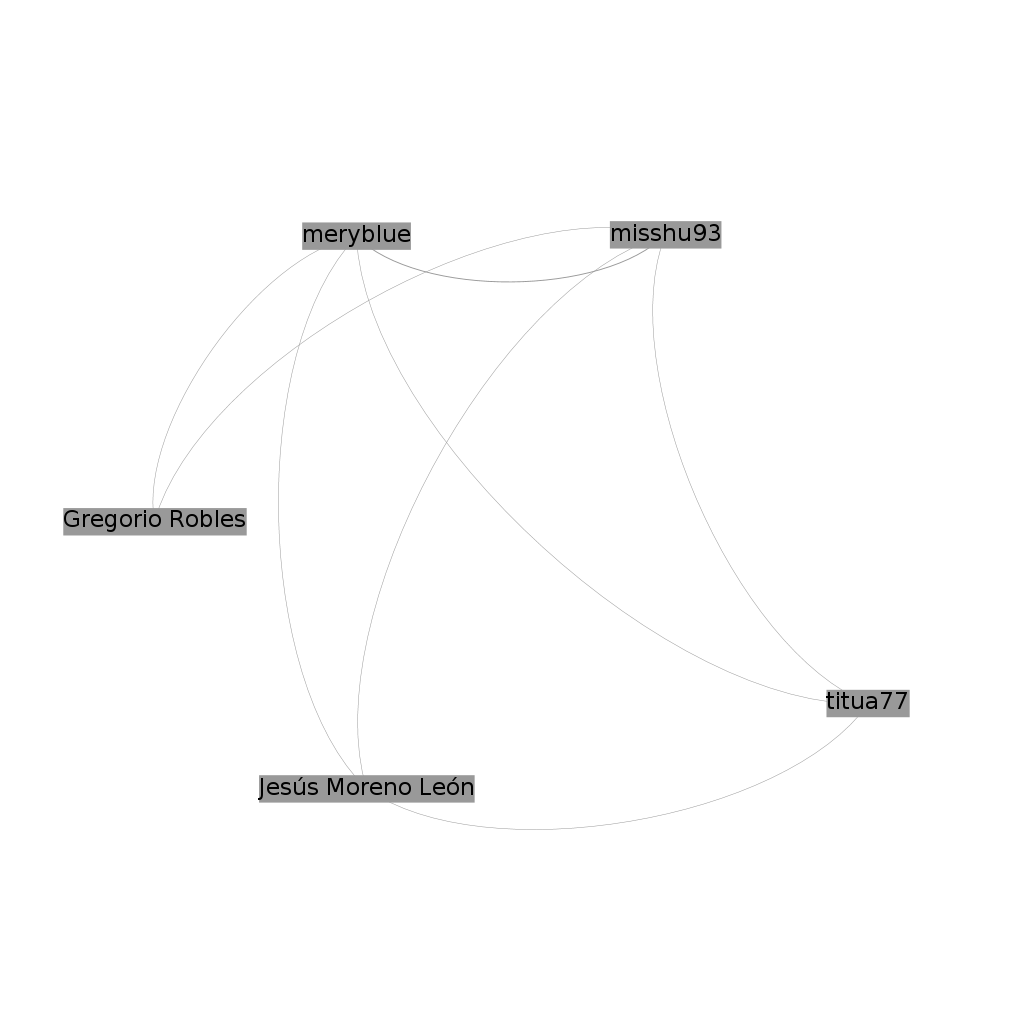
\includegraphics[scale=0.16]{example-graph1.png}
\caption{Collaboration network graph from DrScratch project 
(LibreSoft, Rey Juan Carlos University) - 1st semester, 2015}
\end{figure}
\end{frame}

%------------------------------------------------

\begin{frame}
\frametitle{In these network graphs:}
\begin{block}{Nodes = Developers}
Two developers (nodes) are connected if they have collaborated together.
\end{block}

\begin{block}{Edges = Collaborations}
Edges width represents the amount of collaboration
(The wider the edge is, the greater is the number of interactions between those two nodes).
\end{block}

\end{frame}

%------------------------------------------------

\subsection{New-level analysis} % A subsection can be created just before a set of slides with a common theme to further break down your presentation into chunks

\begin{frame}
\frametitle{Up to now...}
\begin{itemize}
\item In most social network studies the resulting network is based on file/module data.
\item If there is a collaboration between two developers in the same file/module, these developers are connected.
\end{itemize}
\end{frame}

%------------------------------------------------

\begin{frame}
\frametitle{A different point of view}
\begin{itemize}
\item When there are tens of files in a module or thousands of lines in a file, did collaboration really exist?
\item We think the resulting collaboration network graph depends heavily on the granularity level that is considered.
\end{itemize}
\end{frame}

%------------------------------------------------

\begin{frame}
\frametitle{A different point of view: New-level analysis}
\begin{itemize}
\item We've been working to obtain collaboration graphs at function/method level.
\item In these graphs, two developers collaborate if they have modified the same function in a given time period.
\item Excluding large fuctions/methods, we think this new point of view can help us to understand better this analysis.
\end{itemize}
\end{frame}

%------------------------------------------------
\section{Methodology}
\subsection{Building a collaboration graph}
\begin{frame}
\frametitle{Methodology: Our tool}
\begin{itemize}
\item In LibreSoft, our department at Rey Juan Carlos University,
we have developed a python script named GraphDataCreator 
\item This script studies changes in a given 
Git-tracked repository.
\item Using the commit history of all contributors in a specified period of time.
\end{itemize}
\end{frame}
%------------------------------------------------

\subsection{Detailed algorithm}

\begin{frame}
\frametitle{Detailed algorithm I}
\begin{figure}
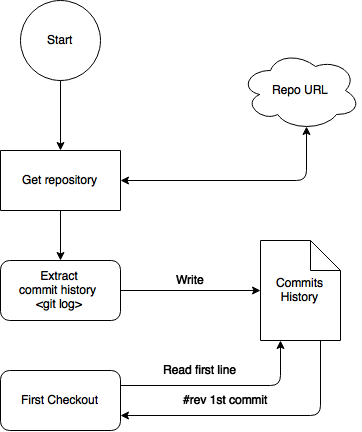
\includegraphics[scale=0.4]{GDCphase1.png} 
\caption{Phase 1 of GraphDataCreator}
\label{fig:phase1}
\end{figure}
\end{frame}

%------------------------------------------------

\begin{frame}
\frametitle{Detailed algorithm II}
\begin{figure}
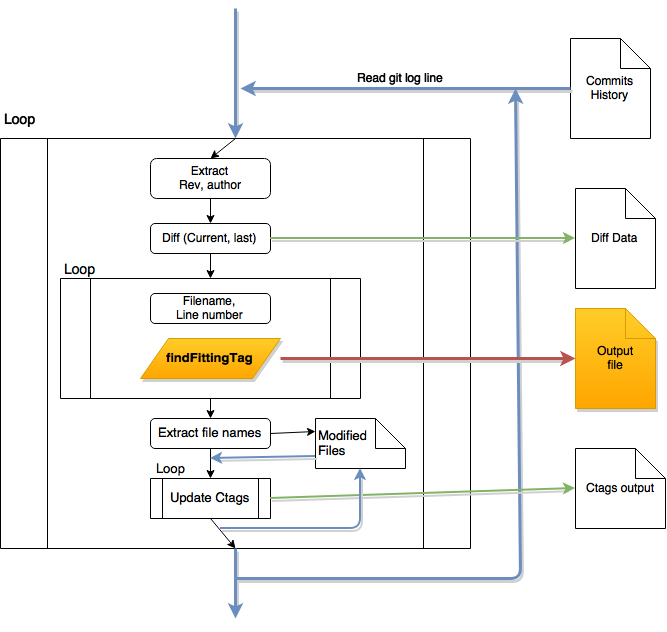
\includegraphics[scale=0.3]{GDCphase2.png} 
\caption{Phase 2 of GraphDataCreator}
\label{fig:phase2}
\end{figure}
\end{frame}

%------------------------------------------------

\begin{frame}
\frametitle{Detailed algorithm: findFittingTag}
\begin{figure}
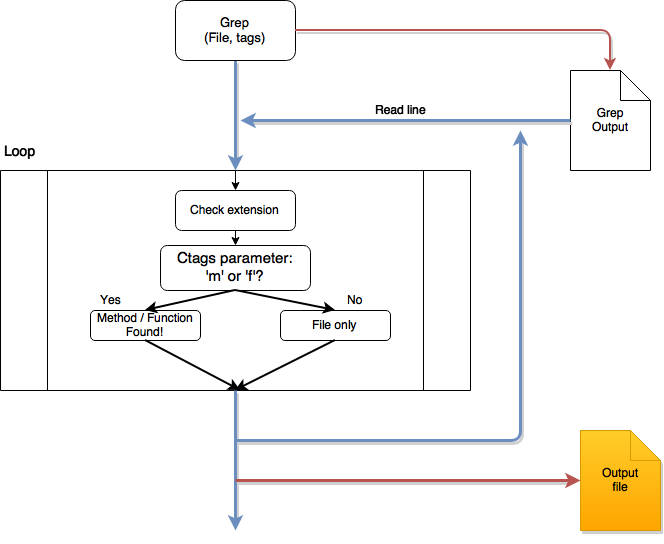
\includegraphics[scale=0.3]{GDCfft.png} 
\caption{Method 'findFittingTag' of GraphDataCreator}
\label{fig:phasefft}
\end{figure}
\end{frame}

%------------------------------------------------

\begin{frame}
\frametitle{Detailed algorithm III}
\begin{figure}
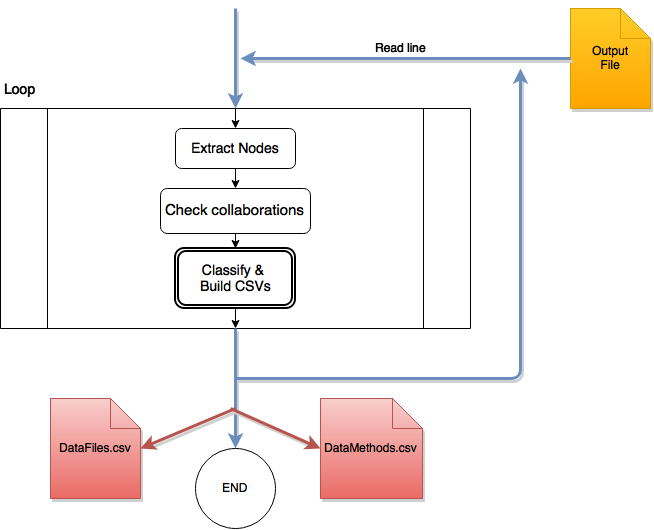
\includegraphics[scale=0.35]{GDCphase3.png} 
\caption{Phase 3 of GraphDataCreator}
\label{fig:phase3}
\end{figure}
\end{frame}

%------------------------------------------------
\section{Case of study}
\subsection{Gedit}
\begin{frame}
\frametitle{Case of study: Gedit}
\begin{itemize}
\item We used the program to study the evolution of GNOME-text editor Gedit.
\item The considered date range for this study goes from the very beginning of the project to this year.
\item To extract data from wide time periods we have developed a super-script that automatically divides large date ranges into smaller periods.
\end{itemize}
\end{frame}

%------------------------------------------------

\begin{frame}
\frametitle{Summing up...}
\begin{block}{Date range}
\begin{itemize}
\item Goes form April 15, 1998 until April 15, 2015. (17 years!)
\item Divided into six-month periods
\end{itemize}
\end{block}

\begin{block}{Resulting data}
\begin{itemize}
\item Two different graphs: for each date range, 
an in-file and an in-method network.
\item Statistic parameters referred to networks, such as betweeness centrality and clustering coefficent.
\end{itemize}
\end{block}

\end{frame}

%------------------------------------------------
\subsubsection{Results}

\begin{frame}
\frametitle{Graphic results: 1st semester, 2001}
\begin{figure}[h!]
\begin{center}
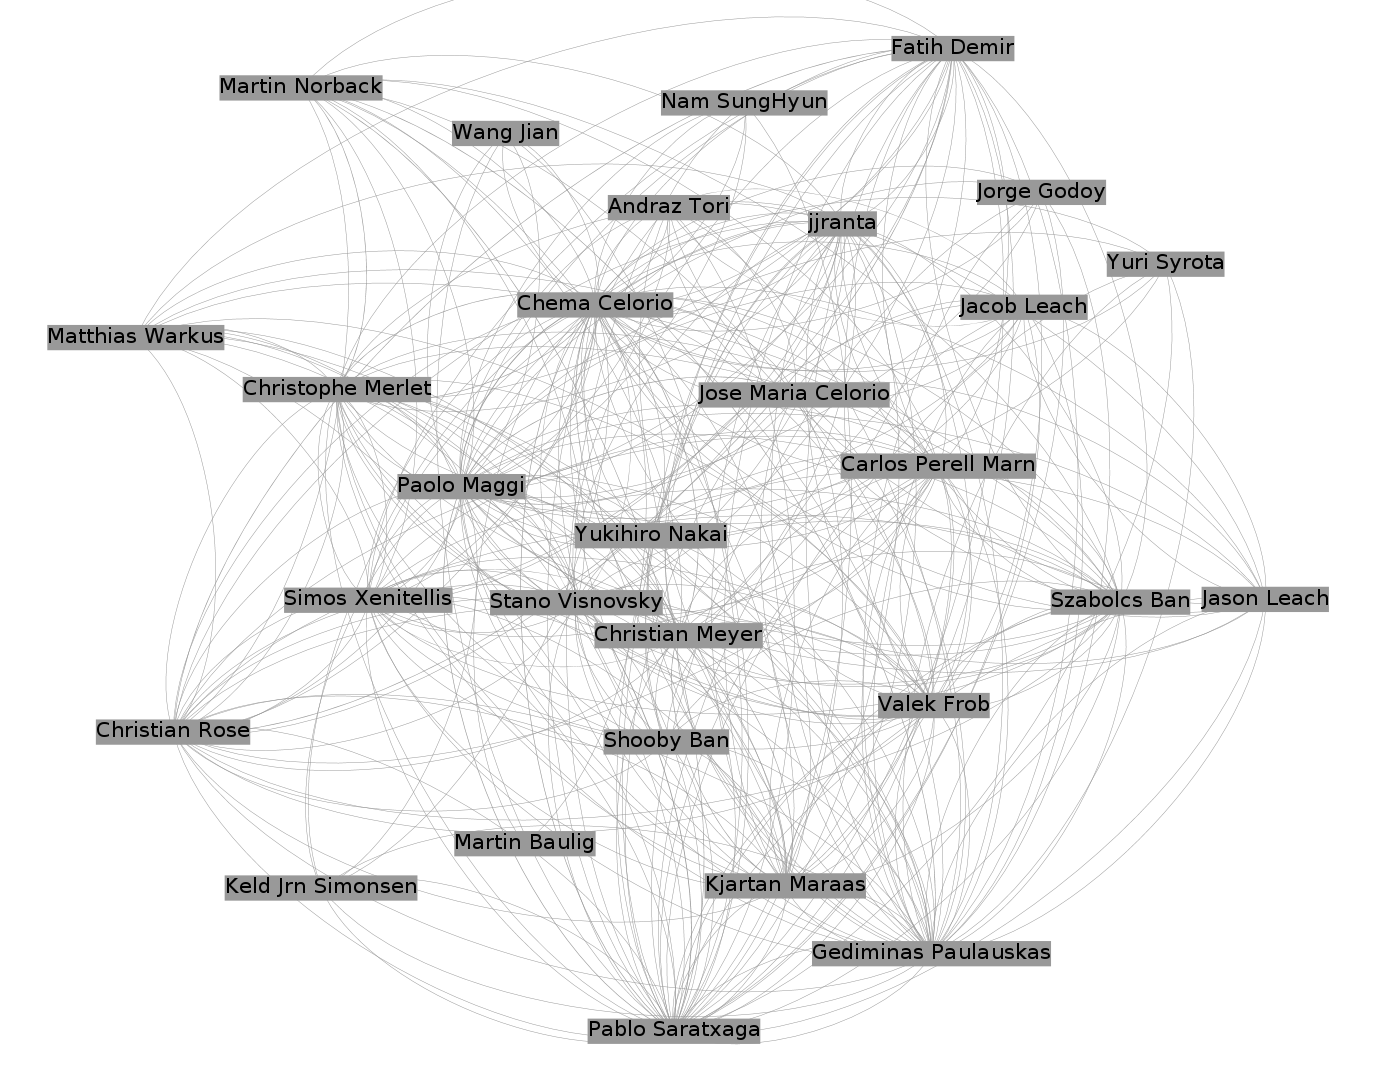
\includegraphics[scale=0.12]{g2001files.png} 
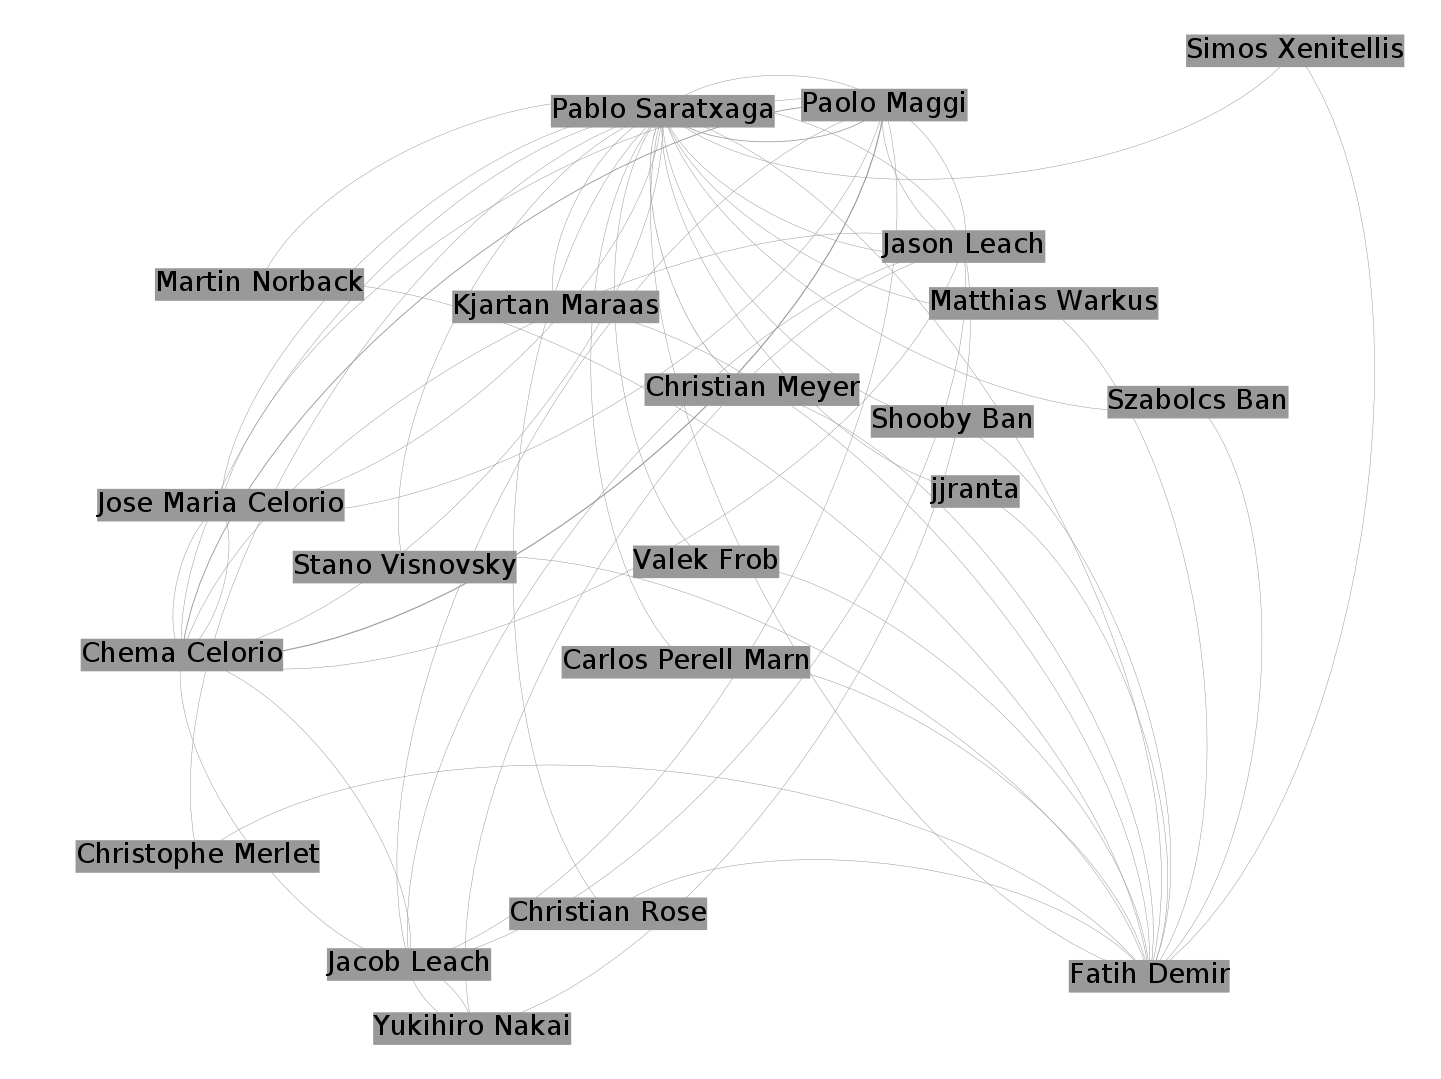
\includegraphics[scale=0.12]{g2001methods.png}
\caption{In-file (left) and In-method (right) collaboration network graphs}
\label{fig:2001}
\end{center}
\end{figure}
\end{frame}

%------------------------------------------------
\begin{frame}
\frametitle{Graphic results: 1st semester, 2014}
\begin{figure}[h!]
\begin{center}
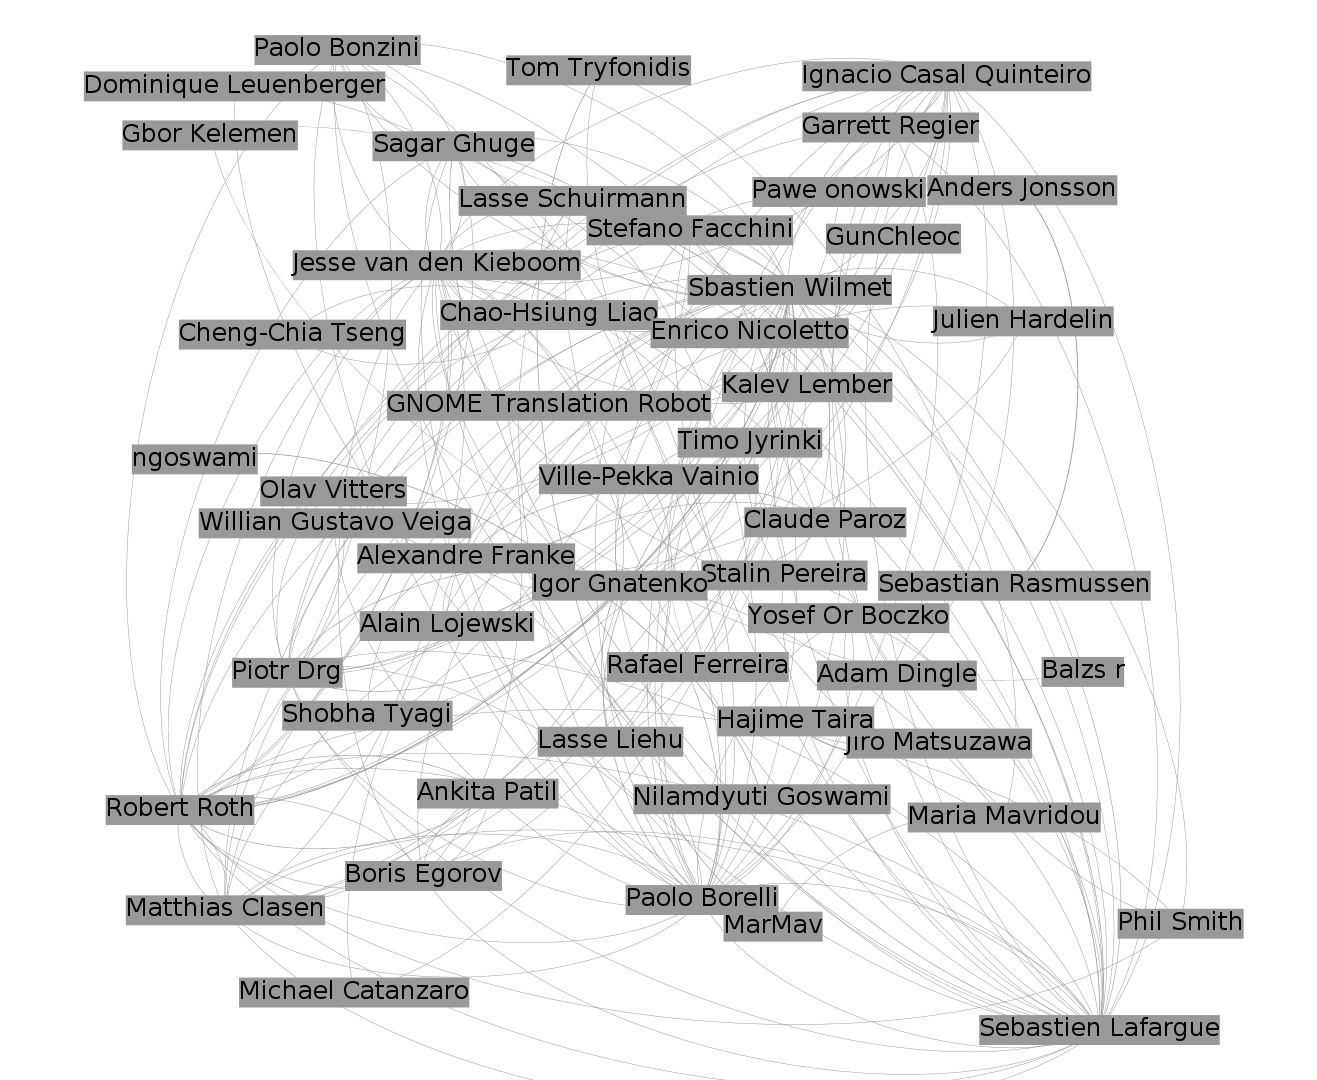
\includegraphics[scale=0.12]{g2014files.png} 
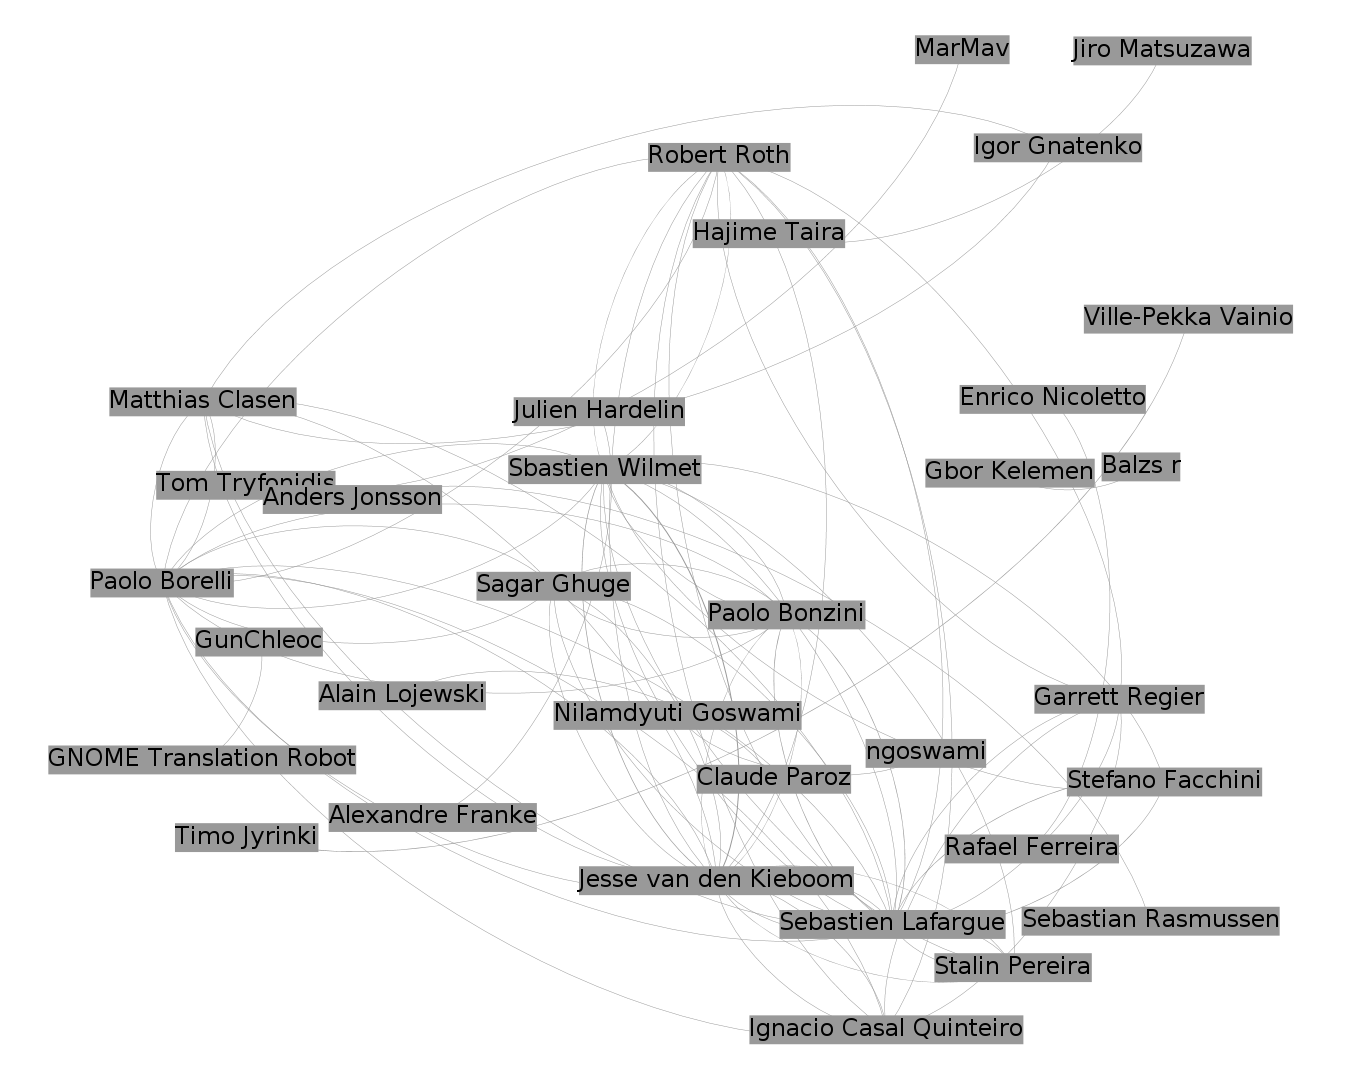
\includegraphics[scale=0.12]{g2014methods.png}
\caption{In-file (left) and In-method (right) collaboration network graphs}
\label{fig:2014}
\end{center}
\end{figure}
\end{frame}

%------------------------------------------------
\begin{frame}
\frametitle{Numeric results: Number of developers}
\begin{figure}
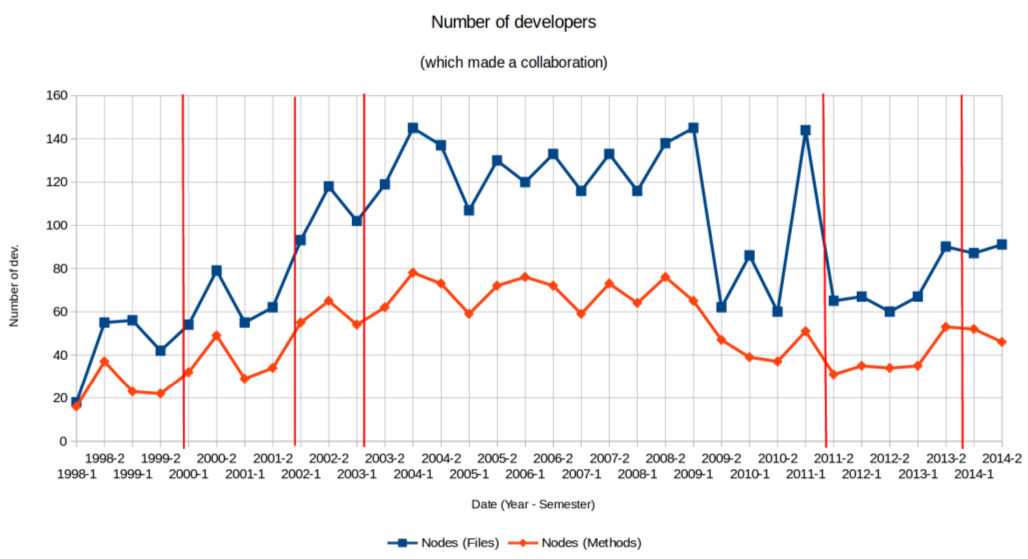
\includegraphics[scale=0.32]{chart1.png}
\label{fig:chartdev1}
\end{figure}
\end{frame}

%------------------------------------------------
\begin{frame}
\frametitle{Numeric results: Number of collaborations}
\begin{figure}
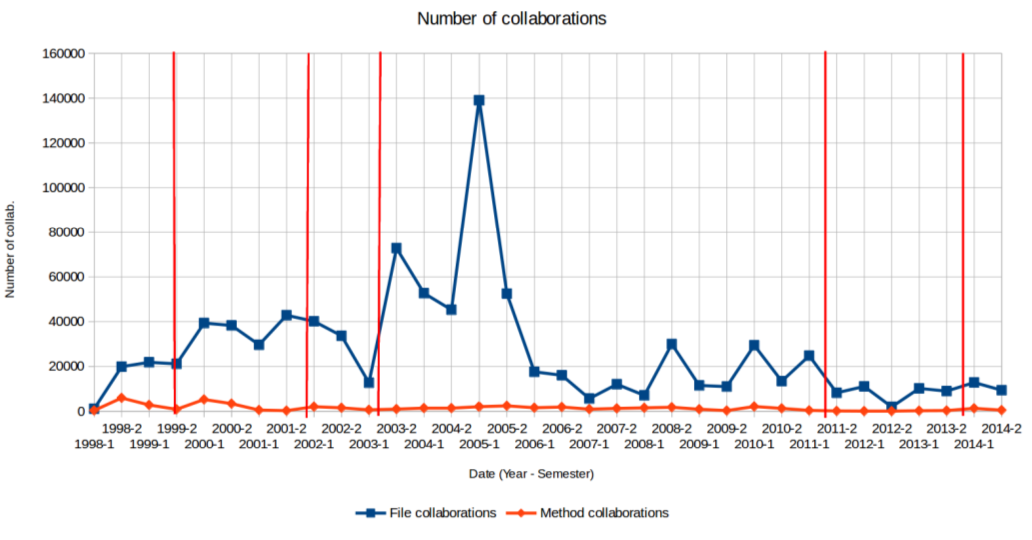
\includegraphics[scale=0.32]{chart2.png}
\label{fig:chartdev2}
\end{figure}
\end{frame}

%------------------------------------------------
\section{Future work}

\begin{frame}
\frametitle{Future work}
\begin{itemize}
% FIXME: Girvan-Newman algorithm?
\item Reproduce some of the studies done in the past now at method/function level.
\item Include algorithms to track function name changes and merge developer aliases.
\item Add developer affiliation information (Examples: projects like OpenStack or WebKit)
\item Improve graph visualization (Girvan-Newman algorithm + taking into account affiliation data)

\end{itemize}
\end{frame}

%------------------------------------------------

\begin{frame}
\frametitle{References}
\footnotesize{
\begin{thebibliography}{99} % Beamer does not support BibTeX so references must be inserted manually as below
\bibitem[Smith, 2012]{p1} John Smith (2012)
\newblock Title of the publication
\newblock \emph{Journal Name} 12(3), 45 -- 678.
\end{thebibliography}
}
\end{frame}

%------------------------------------------------

\begin{frame}
\Huge{\centerline{Any questions?}}
\end{frame}

%------------------------------------------------

\begin{frame}
\Huge{\centerline{Thanks for your attention!}}
\end{frame}

%----------------------------------------------------------------------------------------

\end{document} 